% !TEX encoding = UTF-8 Unicode
\documentclass[BachelorPaper]{subfiles}
\acresetall
%Providecommands für Subfiles
    \providecommand{\citepic}[1]{(#1)}
    \providecommand{\citefig}[2]{(#1, S. #2)}
    \providecommand{\citefigm}[2]{(Modifiziert #1, S. #2)}

\begin{document}
\chapter{Methods}
The following sections include the steps taken to create the BOINSO network applications and the way the distinct components exchange information.

\section{BOINSO Core Web Application}
\label{sec:methods_boinso_core}

\subsection{Core Data Model}
\label{subsec:methods_core_model}

\begin{figure}[!htbp]
\centering
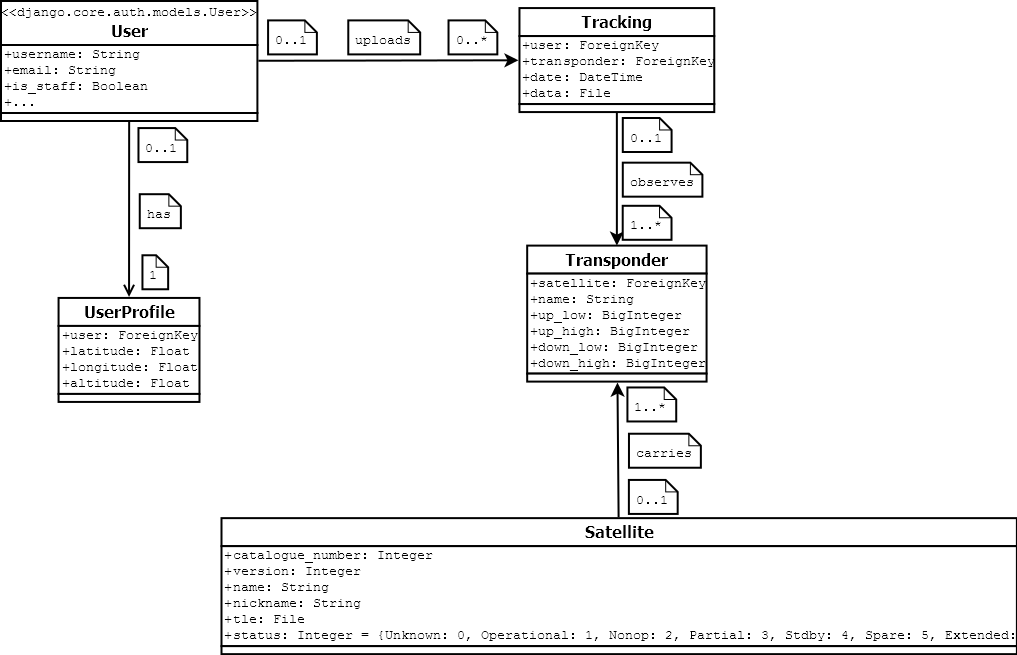
\includegraphics[width=0.9\linewidth]{PICs/diagrams/boinso_core_models.png}
\caption{BOINSO Core Web Application model graph}\label{fig:boinso_core_models}
\end{figure}

As seen in figure \ref{fig:boinso_core_models} the model graph was modeled with only a view important entities as the initial functionality only includes passive satellite passes --  meaning the tracking of a reoccurring transponder transmission. The Django core implementation of the user model was incorporated into the graph as it already included extensive integration in the authentication and permission system. The extension of the user profile was used to add \ac{GCC} related information which offers researches means for statistical segmentation.\\

\subsection{Data model migrations}
\label{subsec:methods_model_migrations}

In order to implement changes to the data model (during initial development as well as the future) Django's migration system was used. The migration system created script files which allowed to make substantial changes to the underlying data source in a portable and retractable manner. A typical migration file as seen in listing \ref{lst:migration} provides semantic naming, chronological enumeration and the possibility to transport model and data changes to all collaborating developers using the common source code repositories.\\

\lstinputlisting[language=Python, caption={BOINSO Core Web Application model migration file including the addition of an integer typed catalogue number field to the satellite model.}, label=lst:migration]{listings/0004_satellite_catalogue_number.py}

\subsection{Web API}
\label{subsec:methods_web_api}

Table \ref{tab:web_api_spec} shows the different \ac{API} endpoints which were implemented to interact with a \ac{MCC} in a programmatic way using \ac{HTTP} verbs. As almost every programming language has a certain amount of networking capabilities being able to make \ac{HTTP} calls it was seen as the most reasonable approach to make the client development as open as possible. In order to make the \ac{API} usable for open scripted clients as well as closed compiled clients an implementation of the OAuth2 authorization framework as stipulated in \cite{rfc6749}.\\

\begin{table}[!htbp]
	\centering
	\begin{tabular}{| l | l | p{3.5cm} | l | l |}
		\hline
		Method & Endpoint & Usage & Returns & Auth \\ \hline
		POST & \url{/api/sign_up/} & Sign up new \ac{GCC} & OAuth2 credentials & None \\ \hline
		GET & \url{/api/login/} & Retrieve registered \ac{GCC} & OAuth2 credentials & HTTP Basic \\ \hline
		GET & \url{/api/satellites/} & Retrieves list of available satellites & Array of satellites & None \\ \hline
		GET & \url{/api/satellites/:id/} & Retrieves satellite with specific ID & Satellite & None \\ \hline
		GET & \url{/api/transponders/:id/} & Retrieves transponder with specific ID & Transponder & None \\ \hline
		GET & \url{/api/user-profiles/} & Retrieves user related to auth token & User profile & OAuth2 \\ \hline
		GET & \url{/api/user-profiles/:id/} & Retrieves user profile with specific ID & User profile & OAuth2 \\ \hline
		PUT/PATCH & \url{/api/user-profiles/:id/} & Updates user profile with ID & User profile & OAuth2 \\ \hline
		DELETE & \url{/api/user-profiles/:id/} & Deletes user profile with specific ID & Deleted Notification & OAuth2 \\ \hline
	\end{tabular}
	\caption{Web API specifications listing method with HTTP-verbs relative endpoint \ac{URL} a short usage note a short description of the returned values and the used authentication type}
	\label{tab:web_api_spec}
\end{table}

In order to keep users relatively independent a user profile (once registered at the \ac{MCC} web application) poses as an application (using the OAuth2 vernacular) making the access to OAuth2 protected endpoints uniform on all client implementation. The OAuth2 provider used in the Boinso Core Web Application was added using the extensive Django OAuth Toolkit distributed under the \ac{BSD} license. Utilizing the capabilities of the provided tools it was possible to both implement the Boinso MCC Web Client as well as the BOINSO GPredict Bridge with a web native callback driven authentication work-flow even though the initial configuration of the BOINSO Core Web Application was considerably more complex.\\

To guarantee a secure transmission of authentication data (login calls require \ac{HTTP} Basic authentication which is relatively easy to decipher while OAuth2 access tokens are not required to be encrypted) a \ac{SSL}/\ac{TLS} encrypted connection should be used. \acp{MCC} can create their own certificates but should also consider investing in signed certificates by accredited institutions. \\

Besides the functionality of the web \ac{API} and its versatile authentication system another feature of the used components include an automatically generated browsable \ac{API}. It was not part of this project to change the design or branding which leads to the \ac{API} root in figure \ref{fig:browsable_api_root} stills showing the Django Rest Framework base style.

\begin{figure}[!htbp]
\centering
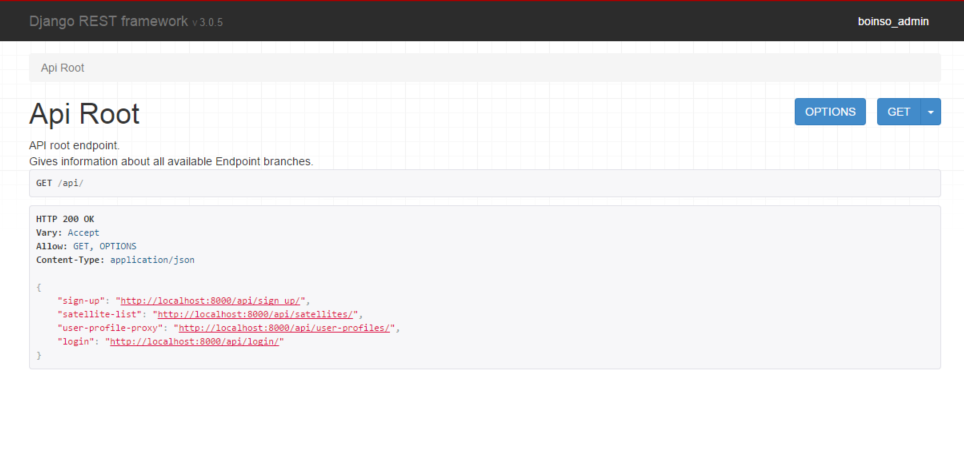
\includegraphics[width=0.96\linewidth]{PICs/BacPics/api_root.png}
\caption{Browsable API root view. API components are interconnected by URLs allowing users both manually as well as programatically discovering API components.}\label{fig:browsable_api_root}
\end{figure}

\section{BOINSO MCC Web Client}
\label{sec:methods_boinso_web}

The BOINSO MCC Web Client was constructed as a sample client implementation, an easy to use and extend web application template for \acp{MCC} and the first interaction point for \acp{GCC}. The main focus was to keep it as simple as possible while giving users a intuitive experience making it possible for them to register with a \ac{MCC}, update their profile information and get informed about the \ac{MCC}'s satellites.\\

Using AngularJS, it's ngResource module and the capabilities of the Django \ac{CORS} Headers module (in the BOINSO Core Web Application) the application was build to request and load user data -- if the authentication process resulted in positive application feedback -- asynchronously and rather than interrupting user commands by alerts in cases of failure redirecting him or her to a state where the problem can be countered.\\

In AngularJS this behavior could be implemented by using \ac{HTTP} interceptor chains like seen in listing \ref{lst:http_interceptor} making extensive use of lazy dependency injection to avoid the risk of circular constructor dependencies.\\

\lstinputlisting[language=JavaScript, caption={Example for a HTTP interceptor reacting to HTTP 401 messages redirecting the user to a log-in overlay.}, label=lst:http_interceptor, firstline=34, lastline=55]{listings/config.js}

\section

\end{document}